
\documentclass{article}
\usepackage{graphicx}
\usepackage{float}
\usepackage{listings}
\usepackage{tabularx}

\title{
\large AFRICAN UNIVERSITY OF SCIENCE \& TECHNOLOGY \\COMPUTER SCIENCE DEPARTMENT\\
\\
\\
Masters Thesis\\
\\
\large FAST AND ACCURATE FEATURE-BASED REGION IDENTIFICATION
}

\date{June 30, 2019}
\begin{document}
 
\begin{titlepage}
\maketitle
\begin{abstract}
\noindent There have been several improvement in object detection and semantic segmentation results in recent years. Baseline systems that drives these advances are Fast/Faster R-CNN, Fully Convolutional Network and recently \textbf{Mask R-CNN} and its variant that has a weight transfer function.  Mask R-CNN is the state-of-art.  This research will extend the application of the state-of-art in object detection and semantic segmentation in drone datasets. Existing drone datasets will be used to learn semantic segmentation on drone images using \textbf{Mask R-CNN}. And a new drone dataset will be collected, labelled, annotated with a bounding box object detection Drone images will be collected with the drone developed by the Robotic team at African University of Science and Technology, Abuja, which will be made public for academic researches.
\\
\\
This work is the result of my own activity. I have neither given nor received unauthorized assistance on this work.
\\
\\

\noindent
\begin{tabular}{lr}
JULY 2019
&
Francis Maduakor
\end{tabular}

\noindent
\begin{tabular}{l}
THESIS SUPERVISOR:\\
PROF. DR. LEHEL CSATÓO \\
FACULTY OF MATHEMATICS AND INFORMATICS, \\
BABES¸ BOLYAI UNIVERSITY OF CLUJ-NAPOCA, ROMANIA 
\end{tabular}








\end{abstract}
\end{titlepage}


\begin{center}
AFRICAN UNIVERSITY OF SCIENCE \& TECHNOLOGY \\
COMPUTER SCIENCE DEPARTMENT \\
Masters Thesis \\
FAST AND ACCURATE FEATURE-BASED REGION IDENTIFICATION\\

\includegraphics{images/logo.jpg}
\end{center}

\noindent
\begin{tabular}{lr}
THESIS SUPERVISOR:	&      STUDENT: 
\end{tabular}

\begin{tabular}{lr}
LEHEL CSATÓO\\ 
FACULTY OF MATHEMATICS AND INFORMATICS,\\
BABES¸ BOLYAI UNIVERSITY OF CLUJ-NAPOCA,\\
ROMANIA
&
Mr. Francis Maduakor
\end{tabular}
•••••••••••
\begin{center}
   JULY 2019 
\end{center}

\clearpage 
\tableofcontents
\clearpage

\section{CHAPTER 1}
\subsection{CHAPTER ON THEORY}
\subsubsection{Image Classification}
Image classification is the process of assigning land cover classes to pixels. Image classification refers to the task of extracting information classes from a multiband raster image. The resulting raster from image classification can be used to create thematic maps. Depending on the interaction between the analyst and the computer during classification, there are two types of classification: supervised and unsupervised. The image classification plays an important role in environmental and socioeconomic applications. In order to improve the classification accuracy, scientists have laid path in developing the advanced classification techniques.
Image classification analyzes the numerical properties of various image features and organizes data into categories. Classification algorithms typically employ two phases of processing: training and testing. In the initial training phase, characteristic properties of typical image features are isolated and, based on these, a unique description of each classification category, i.e. training class, is created. In the subsequent testing phase, these feature-space partitions are used to classify image features. The description of training classes is an extremely important component of the classification process. In supervised classification, statistical processes (i.e. based on an a priori knowledge of probability distribution functions) or distribution-free processes can be used to extract class descriptors. Unsupervised classification relies on clustering algorithms to automatically segment the training data into prototype classes. In either case, the motivating criteria for constructing training classes are that they are:
\begin{enumerate}
\item Independent, e.a change in the description of one training class should not change the value of another,
\item Discriminatory, e.different image features should have significantly different descriptions, and
\item Reliable, all image features within a training group should share the common definitive descriptions of that group.
\end{enumerate}

A convenient way of building a parametric description of this sort is via a feature vector ​v1,v2,………,vn​where ​n​is the number of attributes which describe each image feature and training class. This representation allows us to consider each image feature as occupying a point, and each training class as occupying a sub-space (i.e. a representative point surrounded by some spread, or deviation), within the n-dimensional classification space. Viewed as such, the classification problem is that of determining to which sub-space class each feature vector belongs.
\begin{figure}[H]
  \centering
  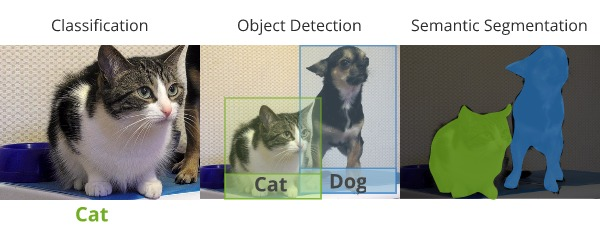
\includegraphics[width=0.7\linewidth]{images/classification_detection_segmentaion_comparisons.jpeg}
   \caption{Image Classification,Object detection Semantic Segmentation.}
\end{figure}
\subsubsection{Object Detection}
 The goal of object detection is to detect all instances of objects from a known
class, such as people, cars or faces in an image. Typically only a small number
of instances of the object are present in the image, but there is a very large
number of possible locations and scales at which they can occur and that need
to somehow be explored.
Each detection is reported with some form of pose information. This could
be as simple as the location of the object, a location and scale, or the extent
of the object defined in terms of a bounding box. In other situations the pose
information is more detailed and contains the parameters of a linear or non-linear
transformation. For example a face detector may compute the locations of the
eyes, nose and mouth, in addition to the bounding box of the face. An example
of a vehicle and person detection that specifies the locations of certain parts is shown in
Figure 1. The pose could also be defined by a three-dimensional transformation
specifying the location of the object relative to the camera.
Object detection systems construct a model for an object class from a set of
training examples. In the case of a fixed rigid object only one example may be
needed, but more generally multiple training examples are necessary to capture
certain aspects of class variability.
\begin{figure}[H]
  \centering
  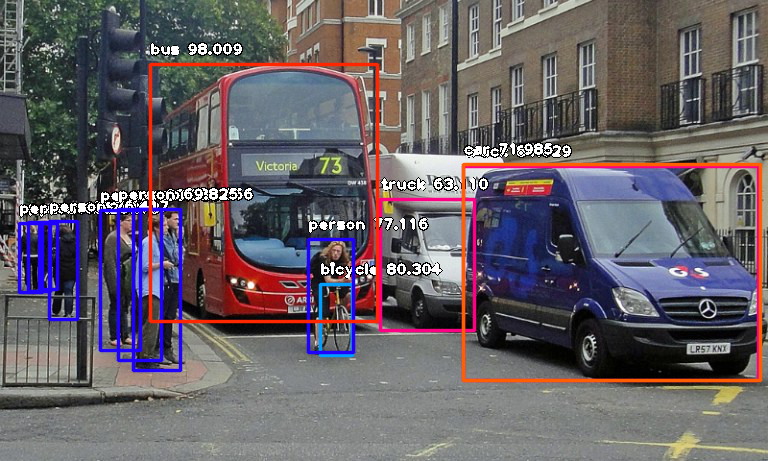
\includegraphics[width=0.5\linewidth]{images/object_det.jpeg}
   \caption{Object detection with bounding boxes.}
\end{figure}

Object detection methods fall into two major categories, generative and discriminative. The first consists of a probability model for the pose variability of the objects together with an appearance model: a probability model for the image appearance conditional on a given pose, together with a model for background, i.e. non-object images. The model parameters can be estimated from training data and the decisions are based on ratios of posterior probabilities. The second typically builds a classifier that can discriminate between images (or sub-images) containing the object and those not containing the object. The parameters of the classifier are selected to minimize mistakes on the training data, often with a regularization bias to avoid overfitting. Other distinctions among detection algorithms have to do with the computational tools used to scan the entire image or search over possible poses, the type of image representation with which the models are constructed, and what type and how much training data is required to build a model.	

%\clearpage




\subsubsection{
Semantic Segmentation
}
Segmentation is essential for image analysis tasks. Semantic segmentation describes the process of associating each pixel of an image with a class label, (such as flower, person, road, sky, ocean, or car).
Semantic image segmentation can be applied effectively to any task that involves the segmentation of visual information. Examples include road segmentation for autonomous vehicles, medical image segmentation, scene segmentation for robot perception, and in image editing tools. Whilst currently available systems provide accurate object recognition, they are unable to delineate the boundaries between objects with the same accuracy.

Oxford researchers have developed a novel neural network component for semantic segmentation that enhances the ability to recognise and delineate objects. This invention can be applied to improve any situation requiring the segmentation of visual information.

Semantic image segmentation plays a crucial role in image understanding, allowing a computer to recognise objects in images. Recognition and delineation of objects is achieved through classification of each pixel in an image. Such processes have a wide range of applications in computer vision, in diverse and growing fields such as vehicle autonomy and medical imaging.

The previous state-of-the-art image segmentation systems used Fully Convolutional Neural Network (FCNN) components, which offer excellent accuracy in recognising objects. Whilst this development represented a significant improvement in semantic segmentation, these networks do not perform well in delineating object boundaries. Conditional Random Fields (CRFs) can be employed in a post-processing step to improve object boundary delineation, however, this is not an optimum solution owing to a lack of integration with the deep network.
\begin{figure}[H]
  \centering
  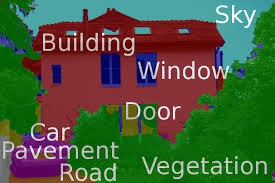
\includegraphics[width=0.5\linewidth]{images/semantic.jpg}
   \caption{Image with semantic segmentation.}
\end{figure}
Oxford researchers have developed a neural network component for semantic segmentation that harnesses the exceptional object recognition of FCNNs and the powerful boundary delineation of CRFs. CRFs are fully integrated as recurrent neural networks, resulting in a system that offers enhanced performance compared to the previous state-of-the-art. The novel system can be applied to any task that involves the segmentation of visual information. Examples include road segmentation for autonomous vehicles, medical image segmentation, scene segmentation for robot perception, and in image editing tools. Oxford University Innovation is seeking industrial partners that wish to explore the use of this system for commercial applications.
\subsubsection{
Instance Segmentation
}
Instance segmentation is one step ahead of semantic segmentation wherein along with pixel level classification, we expect the computer to classify each instance of a class separately. For example in the image above there are 3 people, technically 3 instances of the class “Person”. All the 3 are classified separately (in a different color). But semantic segmentation does not differentiate between the instances of a particular class.
\begin{figure}[H]
  \centering
  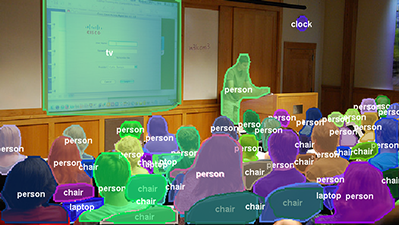
\includegraphics[width=0.5\linewidth]{images/instance.png}
   \caption{Image with instance segmentation.}
\end{figure}
   
   \begin{summary}
  Short description of the specifics...
\end{summary}


%%%%%%%%%%%%%%%%%%%%%%%%%%%%%%%%%%%%%%%%%%%%%%%%%%%%%%%%%%%%%%%%%%%%%%%
\section{Linear discriminant}\label{sec:THEORY:linear}

There is often equation:
\begin{equation}
	f: \Omega_x \rightarrow {\mathbb{R}}
	\quad\text{ such that }
	\quad f(x)
	\begin{cases}
		<0 & \forall x\in Neg \\
		\geq 0 & \forall x\in Poz
	\end{cases}
	\label{eq:diszkr:fugg}
\end{equation}



If an equation is not very important, one can use the \$\$ notation...

$$D_k(x)=\tilde{x}^T\alpha_k=\alpha_k^T\tilde{x},$$














 

\end{document}
